% Options for packages loaded elsewhere
\PassOptionsToPackage{unicode}{hyperref}
\PassOptionsToPackage{hyphens}{url}
\PassOptionsToPackage{dvipsnames,svgnames,x11names}{xcolor}
\documentclass[
  10pt,
]{extarticle}
\usepackage{xcolor}
\usepackage[top=1.5in, bottom=1.5in, left=1.5in, right=1.5in]{geometry}
\usepackage{amsmath,amssymb}
\setcounter{secnumdepth}{5}
\usepackage{iftex}
\ifPDFTeX
  \usepackage[T1]{fontenc}
  \usepackage[utf8]{inputenc}
  \usepackage{textcomp} % provide euro and other symbols
\else % if luatex or xetex
  \usepackage{unicode-math} % this also loads fontspec
  \defaultfontfeatures{Scale=MatchLowercase}
  \defaultfontfeatures[\rmfamily]{Ligatures=TeX,Scale=1}
\fi
\usepackage{lmodern}
\ifPDFTeX\else
  % xetex/luatex font selection
\fi
% Use upquote if available, for straight quotes in verbatim environments
\IfFileExists{upquote.sty}{\usepackage{upquote}}{}
\IfFileExists{microtype.sty}{% use microtype if available
  \usepackage[]{microtype}
  \UseMicrotypeSet[protrusion]{basicmath} % disable protrusion for tt fonts
}{}
\makeatletter
\@ifundefined{KOMAClassName}{% if non-KOMA class
  \IfFileExists{parskip.sty}{%
    \usepackage{parskip}
  }{% else
    \setlength{\parindent}{0pt}
    \setlength{\parskip}{6pt plus 2pt minus 1pt}}
}{% if KOMA class
  \KOMAoptions{parskip=half}}
\makeatother
\usepackage{color}
\usepackage{fancyvrb}
\newcommand{\VerbBar}{|}
\newcommand{\VERB}{\Verb[commandchars=\\\{\}]}
\DefineVerbatimEnvironment{Highlighting}{Verbatim}{commandchars=\\\{\}}
% Add ',fontsize=\small' for more characters per line
\usepackage{framed}
\definecolor{shadecolor}{RGB}{248,248,248}
\newenvironment{Shaded}{\begin{snugshade}}{\end{snugshade}}
\newcommand{\AlertTok}[1]{\textcolor[rgb]{0.94,0.16,0.16}{#1}}
\newcommand{\AnnotationTok}[1]{\textcolor[rgb]{0.56,0.35,0.01}{\textbf{\textit{#1}}}}
\newcommand{\AttributeTok}[1]{\textcolor[rgb]{0.13,0.29,0.53}{#1}}
\newcommand{\BaseNTok}[1]{\textcolor[rgb]{0.00,0.00,0.81}{#1}}
\newcommand{\BuiltInTok}[1]{#1}
\newcommand{\CharTok}[1]{\textcolor[rgb]{0.31,0.60,0.02}{#1}}
\newcommand{\CommentTok}[1]{\textcolor[rgb]{0.56,0.35,0.01}{\textit{#1}}}
\newcommand{\CommentVarTok}[1]{\textcolor[rgb]{0.56,0.35,0.01}{\textbf{\textit{#1}}}}
\newcommand{\ConstantTok}[1]{\textcolor[rgb]{0.56,0.35,0.01}{#1}}
\newcommand{\ControlFlowTok}[1]{\textcolor[rgb]{0.13,0.29,0.53}{\textbf{#1}}}
\newcommand{\DataTypeTok}[1]{\textcolor[rgb]{0.13,0.29,0.53}{#1}}
\newcommand{\DecValTok}[1]{\textcolor[rgb]{0.00,0.00,0.81}{#1}}
\newcommand{\DocumentationTok}[1]{\textcolor[rgb]{0.56,0.35,0.01}{\textbf{\textit{#1}}}}
\newcommand{\ErrorTok}[1]{\textcolor[rgb]{0.64,0.00,0.00}{\textbf{#1}}}
\newcommand{\ExtensionTok}[1]{#1}
\newcommand{\FloatTok}[1]{\textcolor[rgb]{0.00,0.00,0.81}{#1}}
\newcommand{\FunctionTok}[1]{\textcolor[rgb]{0.13,0.29,0.53}{\textbf{#1}}}
\newcommand{\ImportTok}[1]{#1}
\newcommand{\InformationTok}[1]{\textcolor[rgb]{0.56,0.35,0.01}{\textbf{\textit{#1}}}}
\newcommand{\KeywordTok}[1]{\textcolor[rgb]{0.13,0.29,0.53}{\textbf{#1}}}
\newcommand{\NormalTok}[1]{#1}
\newcommand{\OperatorTok}[1]{\textcolor[rgb]{0.81,0.36,0.00}{\textbf{#1}}}
\newcommand{\OtherTok}[1]{\textcolor[rgb]{0.56,0.35,0.01}{#1}}
\newcommand{\PreprocessorTok}[1]{\textcolor[rgb]{0.56,0.35,0.01}{\textit{#1}}}
\newcommand{\RegionMarkerTok}[1]{#1}
\newcommand{\SpecialCharTok}[1]{\textcolor[rgb]{0.81,0.36,0.00}{\textbf{#1}}}
\newcommand{\SpecialStringTok}[1]{\textcolor[rgb]{0.31,0.60,0.02}{#1}}
\newcommand{\StringTok}[1]{\textcolor[rgb]{0.31,0.60,0.02}{#1}}
\newcommand{\VariableTok}[1]{\textcolor[rgb]{0.00,0.00,0.00}{#1}}
\newcommand{\VerbatimStringTok}[1]{\textcolor[rgb]{0.31,0.60,0.02}{#1}}
\newcommand{\WarningTok}[1]{\textcolor[rgb]{0.56,0.35,0.01}{\textbf{\textit{#1}}}}
\usepackage{longtable,booktabs,array}
\usepackage{calc} % for calculating minipage widths
% Correct order of tables after \paragraph or \subparagraph
\usepackage{etoolbox}
\makeatletter
\patchcmd\longtable{\par}{\if@noskipsec\mbox{}\fi\par}{}{}
\makeatother
% Allow footnotes in longtable head/foot
\IfFileExists{footnotehyper.sty}{\usepackage{footnotehyper}}{\usepackage{footnote}}
\makesavenoteenv{longtable}
\usepackage{graphicx}
\makeatletter
\newsavebox\pandoc@box
\newcommand*\pandocbounded[1]{% scales image to fit in text height/width
  \sbox\pandoc@box{#1}%
  \Gscale@div\@tempa{\textheight}{\dimexpr\ht\pandoc@box+\dp\pandoc@box\relax}%
  \Gscale@div\@tempb{\linewidth}{\wd\pandoc@box}%
  \ifdim\@tempb\p@<\@tempa\p@\let\@tempa\@tempb\fi% select the smaller of both
  \ifdim\@tempa\p@<\p@\scalebox{\@tempa}{\usebox\pandoc@box}%
  \else\usebox{\pandoc@box}%
  \fi%
}
% Set default figure placement to htbp
\def\fps@figure{htbp}
\makeatother
\setlength{\emergencystretch}{3em} % prevent overfull lines
\providecommand{\tightlist}{%
  \setlength{\itemsep}{0pt}\setlength{\parskip}{0pt}}
\usepackage{xcolor}
\usepackage{hyperref}
\hypersetup{colorlinks=true, linkcolor=blue, urlcolor=blue, citecolor=blue}
\usepackage{float}
\usepackage{fvextra}
\usepackage{fancyhdr}
\usepackage{lastpage}
\usepackage{soul}
\usepackage{etoolbox}
\usepackage{microtype}
\usepackage{tcolorbox}
\usepackage{enumitem}
\usepackage{fancyvrb}
\usepackage{xspace}
\allowdisplaybreaks
\setcounter{tocdepth}{2}
\setcounter{secnumdepth}{0}
\floatplacement{figure}{H}
\makeatletter
\newcommand{\@subtitle}{}
\newcommand{\subtitle}[1]{\gdef\@subtitle{#1}}
\newcommand{\DocSubtitle}{\@subtitle}
\renewcommand{\maketitle}{
  \thispagestyle{plain}
  \null
  \vfill
  \begin{center}
    {\Large \textsc{\@title} \par}\vskip 0.5em
    {\LARGE \bfseries \@subtitle \par}\vskip 0.75em
    {\large \@author \par}\vskip 0.5em
    {\normalsize \@date \par}
  \end{center}
  \vfill
  \tableofcontents
  \vspace{1em}
  \clearpage
}
\AfterEndEnvironment{Highlighting}{\setcounter{CodeLine}{\numexpr\value{CodeLine}+\FV@CodeLineNo\relax}}
\makeatother
\fancypagestyle{plain}{
  \fancyhf{}
  \renewcommand{\headrulewidth}{0pt}
  \renewcommand{\footrulewidth}{0pt}
}
\pagestyle{fancy}
\fancyhf{}
\fancyfoot[C]{\small\textsc{Page}~\thepage~\textsc{of}~\pageref{LastPage}}
\fancyhead[L]{\textsc{Rento Saijo}}
\fancyhead[R]{\textsc{\DocSubtitle}}
\fancyhead[C]{\textsc{\rightmark}}
\renewcommand{\headrulewidth}{0.5pt}
\renewcommand{\footrulewidth}{0.5pt}
\newcounter{CodeLine}
\newcounter{cell}
\AtBeginEnvironment{Highlighting}{\stepcounter{cell}}
\DefineVerbatimEnvironment{Highlighting}{Verbatim}{
  frame=single,
  rulecolor=\color{black},
  framesep=2mm,
  label=\footnotesize Cell \thecell,
  labelposition=topline,
  commandchars=\\\{\},
  breaklines=true,
  breakanywhere=false,
  breaksymbol={},
  numbers=left,
  numbersep=3pt,
  firstnumber=\numexpr\value{CodeLine}+1\relax,
  fontsize=\small
}
\DefineVerbatimEnvironment{verbatim}{Verbatim}{
  breaklines=true,
  breakanywhere=true,
  numbers=left,
  numbersep=3pt,
  firstnumber=1,
  fontsize=\footnotesize
}
\newtcolorbox{problem}[1][]{
  title={\textsc{#1}}
}
\renewcommand{\contentsname}{Table of Contents}
\newcommand{\E}{\mathrm{E}}
\newcommand{\Var}{\mathrm{Var}}
\newcommand{\Cov}{\mathrm{Cov}}
\newcommand{\R}{\textsf{R}\xspace}
\newcommand{\SD}{\mathrm{SD}}
\newcommand{\SE}{\mathrm{SE}}
\usepackage{bookmark}
\IfFileExists{xurl.sty}{\usepackage{xurl}}{} % add URL line breaks if available
\urlstyle{same}
\hypersetup{
  pdftitle={STA 209: Introduction to Time Series Analysis},
  colorlinks=true,
  linkcolor={blue},
  filecolor={Maroon},
  citecolor={blue},
  urlcolor={blue},
  pdfcreator={LaTeX via pandoc}}

\title{STA 209: Introduction to Time Series Analysis}
\usepackage{etoolbox}
\makeatletter
\providecommand{\subtitle}[1]{% add subtitle to \maketitle
  \apptocmd{\@title}{\par {\large #1 \par}}{}{}
}
\makeatother
\subtitle{Homework 5}
\author{Rento Saijo}
\date{April 6, 2026}

\begin{document}
\maketitle

\section{Disclosure}\label{disclosure}

GPT-5.4 Codex was used to create the \texttt{YAML} portion and some \texttt{LaTeX} code to format the text/equations nicely. Page formatting code was also provided by Derin Gezgin. In the setup chunk, chunk options were set for the document and simple helper functions were defined for tables and ACF plots.

\newpage

\section{Problem 1}\label{problem-1}

\begin{problem}[Problem-1 (20 points)]
Suppose a time series follows the following model:
\[
X_t = W_t - 0.2W_{t-2},
\]
where \(W_t \sim WN(0,\sigma_w^2)\), that is, \(\{W_t\}\) is a white noise with mean \(0\) and variance \(\sigma_w^2\).
\begin{enumerate}[label=(\alph*)]
\item Determine its mean.
\item Determine its Auto-Covariance Function (ACVF).
\item Find and plot the Auto-Correlation Function (ACF).
\item Is the process stationary, justify?
\end{enumerate}
\end{problem}

\newpage

\subsection{Problem 1 (a)}\label{problem-1-a}

\begin{problem}[Problem 1 (a)]
Determine its mean.
\end{problem}

Using the linearity of expectation and the fact that \(\mathrm{E}(W_t)=0\) for white noise,
\[
\begin{aligned}
\mathrm{E}(X_t)
&= \mathrm{E}(W_t - 0.2W_{t-2}) \\
&= \mathrm{E}(W_t) - 0.2\mathrm{E}(W_{t-2}) \\
&= 0 - 0.2(0) \\
&= 0.
\end{aligned}
\]

Hence,
\[
\mu_X(t) = \mu_X = 0,
\]
which is not a function of time \(t\).

\newpage

\subsection{Problem 1 (b)}\label{problem-1-b}

\begin{problem}[Problem 1 (b)]
Determine its Auto-Covariance Function (ACVF).
\end{problem}

For all integers \(h\),
\[
\gamma_X(t,h) = \mathrm{Cov}(X_{t+h},X_t) = \mathrm{E}[(X_{t+h}-\mu_{t+h})(X_t-\mu_t)].
\]
Since \(\mu_t = \mu_{t+h} = 0\),
\[
\begin{aligned}
\gamma_X(t,h)
&= \mathrm{E}(X_{t+h}X_t) \\
&= \mathrm{E}[(W_{t+h} - 0.2W_{t+h-2})(W_t - 0.2W_{t-2})] \\
&= \mathrm{E}(W_{t+h}W_t)
   - 0.2\mathrm{E}(W_{t+h}W_{t-2})
   - 0.2\mathrm{E}(W_{t+h-2}W_t)
   + 0.04\mathrm{E}(W_{t+h-2}W_{t-2}).
\end{aligned}
\]

Because \(\{W_t\}\) is white noise with mean \(0\),
\[
\mathrm{E}(W_aW_b) =
\begin{cases}
\sigma_w^2, & a=b,\\
0, & a \neq b.
\end{cases}
\]

Now, let us evaluate the expression case-by-case. If \(h=0\), then
\[
\begin{aligned}
\gamma_X(t,0)
&= \mathrm{E}(W_t^2)
   - 0.2\mathrm{E}(W_tW_{t-2})
   - 0.2\mathrm{E}(W_{t-2}W_t)
   + 0.04\mathrm{E}(W_{t-2}^2) \\
&= \sigma_w^2 - 0 - 0 + 0.04\sigma_w^2 \\
&= 1.04\sigma_w^2.
\end{aligned}
\]

If \(h=2\), then
\[
\begin{aligned}
\gamma_X(t,2)
&= \mathrm{E}(W_{t+2}W_t)
   - 0.2\mathrm{E}(W_{t+2}W_{t-2})
   - 0.2\mathrm{E}(W_tW_t)
   + 0.04\mathrm{E}(W_tW_{t-2}) \\
&= 0 - 0 - 0.2\sigma_w^2 + 0 \\
&= -0.2\sigma_w^2.
\end{aligned}
\]

If \(h=-2\), then
\[
\begin{aligned}
\gamma_X(t,-2)
&= \mathrm{E}(W_{t-2}W_t)
   - 0.2\mathrm{E}(W_{t-2}W_{t-2})
   - 0.2\mathrm{E}(W_{t-4}W_t)
   + 0.04\mathrm{E}(W_{t-4}W_{t-2}) \\
&= 0 - 0.2\sigma_w^2 - 0 + 0 \\
&= -0.2\sigma_w^2.
\end{aligned}
\]

If \(h \neq 0,\pm2\), then none of the time indices match, so every expectation is \(0\). Therefore,
\[
\gamma_X(t,h) = 0.
\]

Hence, the ACVF is
\[
\gamma_X(h) =
\begin{cases}
1.04\sigma_w^2, & h=0,\\
-0.2\sigma_w^2, & h=\pm2,\\
0, & h \in \mathbb{Z}\setminus\{0,-2,2\}.
\end{cases}
\]

This depends only on the lag \(h\), not on time \(t\).

\newpage

\subsection{Problem 1 (c)}\label{problem-1-c}

\begin{problem}[Problem 1 (c)]
Find and plot the Auto-Correlation Function (ACF).
\end{problem}

By definition,
\[
\rho_X(h) = \frac{\gamma_X(h)}{\gamma_X(0)}.
\]
Since \(\gamma_X(0)=1.04\sigma_w^2\),
\[
\rho_X(h) =
\begin{cases}
1, & h=0,\\
\dfrac{-0.2\sigma_w^2}{1.04\sigma_w^2} = -\dfrac{0.2}{1.04} = -\dfrac{5}{26} \approx -0.1923, & h=\pm2,\\
0, & h \in \mathbb{Z}\setminus\{0,-2,2\}.
\end{cases}
\]

So the ACF has one spike of height \(1\) at lag \(0\), two negative spikes of height \(-5/26 \approx -0.1923\) at lags \(-2\) and \(2\), and \(0\) at every other lag.

\begin{Shaded}
\begin{Highlighting}[]
\CommentTok{\# Numerical ACF values used for plotting.}
\NormalTok{p1\_lags }\OtherTok{\textless{}{-}} \SpecialCharTok{{-}}\DecValTok{10}\SpecialCharTok{:}\DecValTok{10}
\NormalTok{p1\_gamma\_over\_sigma2 }\OtherTok{\textless{}{-}} \FunctionTok{ifelse}\NormalTok{(}
\NormalTok{  p1\_lags }\SpecialCharTok{==} \DecValTok{0}\NormalTok{,}
  \FloatTok{1.04}\NormalTok{,}
  \FunctionTok{ifelse}\NormalTok{(}\FunctionTok{abs}\NormalTok{(p1\_lags) }\SpecialCharTok{==} \DecValTok{2}\NormalTok{, }\SpecialCharTok{{-}}\FloatTok{0.2}\NormalTok{, }\DecValTok{0}\NormalTok{)}
\NormalTok{)}
\NormalTok{p1\_rho }\OtherTok{\textless{}{-}}\NormalTok{ p1\_gamma\_over\_sigma2 }\SpecialCharTok{/} \FloatTok{1.04}

\CommentTok{\# Plot the ACF.}
\FunctionTok{acf\_stem\_plot}\NormalTok{(p1\_lags, p1\_rho, }\StringTok{\textquotesingle{}Problem 1: ACF\textquotesingle{}}\NormalTok{)}
\end{Highlighting}
\end{Shaded}

\begin{center}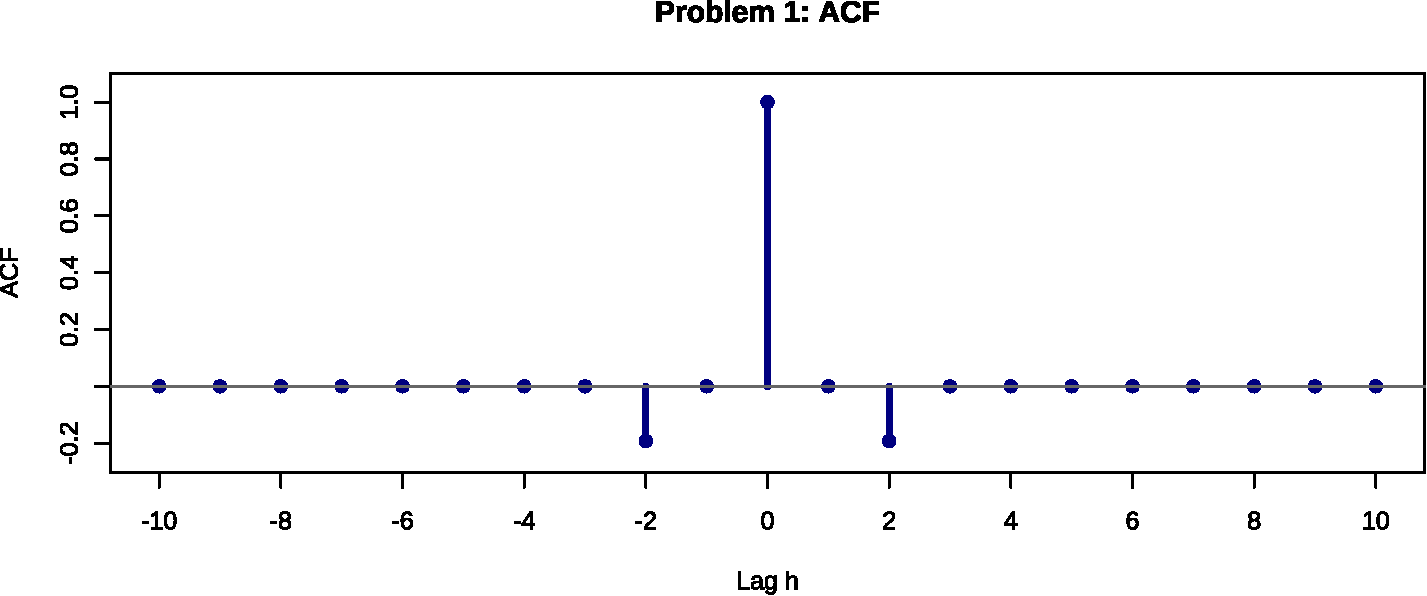
\includegraphics[width=\linewidth]{Homework5_files/figure-latex/unnamed-chunk-2-1} \end{center}

\newpage

\subsection{Problem 1 (d)}\label{problem-1-d}

\begin{problem}[Problem 1 (d)]
Is the process stationary, justify?
\end{problem}

Yes, \(\{X_t\}\) is weakly stationary because of the following:

\begin{enumerate}
\def\labelenumi{\arabic{enumi}.}
\item
  The mean function is independent of time:
  \[
  \mu_X(t) = 0 = \mu_X.
  \]
\item
  The autocovariance function depends only on lag \(h\):
  \[
  \gamma_X(t,h) = \gamma_X(h) =
  \begin{cases}
  1.04\sigma_w^2, & h=0,\\
  -0.2\sigma_w^2, & h=\pm2,\\
  0, & h \in \mathbb{Z}\setminus\{0,-2,2\}.
  \end{cases}
  \]
\end{enumerate}

At lag \(h=0\), the ACVF is the variance, so
\[
\sigma_X^2(t) = \sigma_X^2 = \gamma_X(0) = 1.04\sigma_w^2,
\]
which is also constant over time. Therefore, the process satisfies both conditions for weak stationarity. Hence, \(\{X_t\}\) is stationary.

\newpage

\section{Problem 2}\label{problem-2}

\begin{problem}[Problem 2 (30 points)]
For the following MA process
\[
X_t = W_{t-1} + 2W_t + W_{t+1}
\]
\begin{enumerate}[label=(\alph*)]
\item Determine its mean.
\item Determine its Auto-Covariance Function (ACVF).
\item Find and plot the Auto-Correlation Function (ACF).
\item Is the process stationary, justify?
\end{enumerate}
\end{problem}

\newpage

\subsection{Problem 2 (a)}\label{problem-2-a}

\begin{problem}[Problem 2 (a)]
Determine its mean.
\end{problem}

Using the linearity of expectation and the fact that \(\mathrm{E}(W_t)=0\),
\[
\begin{aligned}
\mathrm{E}(X_t)
&= \mathrm{E}(W_{t-1} + 2W_t + W_{t+1}) \\
&= \mathrm{E}(W_{t-1}) + 2\mathrm{E}(W_t) + \mathrm{E}(W_{t+1}) \\
&= 0 + 2(0) + 0 \\
&= 0.
\end{aligned}
\]

Hence,
\[
\mu_X(t) = \mu_X = 0,
\]
which is not a function of time \(t\).

\newpage

\subsection{Problem 2 (b)}\label{problem-2-b}

\begin{problem}[Problem 2 (b)]
Determine its Auto-Covariance Function (ACVF).
\end{problem}

For all integers \(h\),
\[
\gamma_X(t,h) = \mathrm{Cov}(X_{t+h},X_t) = \mathrm{E}[(X_{t+h}-\mu_{t+h})(X_t-\mu_t)].
\]
Since \(\mu_t = \mu_{t+h} = 0\),
\[
\gamma_X(t,h) = \mathrm{E}(X_{t+h}X_t).
\]
Also,
\[
X_{t+h} = W_{t+h-1} + 2W_{t+h} + W_{t+h+1}.
\]
Therefore,
\[
\begin{aligned}
\gamma_X(t,h)
&= \mathrm{E}[(W_{t+h-1} + 2W_{t+h} + W_{t+h+1})(W_{t-1} + 2W_t + W_{t+1})] \\
&= \mathrm{E}(W_{t+h-1}W_{t-1})
 + 2\mathrm{E}(W_{t+h-1}W_t)
 + \mathrm{E}(W_{t+h-1}W_{t+1}) \\
&\quad + 2\mathrm{E}(W_{t+h}W_{t-1})
 + 4\mathrm{E}(W_{t+h}W_t)
 + 2\mathrm{E}(W_{t+h}W_{t+1}) \\
&\quad + \mathrm{E}(W_{t+h+1}W_{t-1})
 + 2\mathrm{E}(W_{t+h+1}W_t)
 + \mathrm{E}(W_{t+h+1}W_{t+1}).
\end{aligned}
\]

Again, since \(\{W_t\}\) is white noise,
\[
\mathrm{E}(W_aW_b) =
\begin{cases}
\sigma_w^2, & a=b,\\
0, & a \neq b.
\end{cases}
\]

Now evaluate case-by-case. If \(h=0\), then
\[
\begin{aligned}
\gamma_X(t,0)
&= \mathrm{E}(W_{t-1}^2)
 + 2\mathrm{E}(W_{t-1}W_t)
 + \mathrm{E}(W_{t-1}W_{t+1}) \\
&\quad + 2\mathrm{E}(W_tW_{t-1})
 + 4\mathrm{E}(W_t^2)
 + 2\mathrm{E}(W_tW_{t+1}) \\
&\quad + \mathrm{E}(W_{t+1}W_{t-1})
 + 2\mathrm{E}(W_{t+1}W_t)
 + \mathrm{E}(W_{t+1}^2) \\
&= \sigma_w^2 + 0 + 0 + 0 + 4\sigma_w^2 + 0 + 0 + 0 + \sigma_w^2 \\
&= 6\sigma_w^2.
\end{aligned}
\]

If \(h=1\), then
\[
\begin{aligned}
\gamma_X(t,1)
&= \mathrm{E}(W_tW_{t-1})
 + 2\mathrm{E}(W_tW_t)
 + \mathrm{E}(W_tW_{t+1}) \\
&\quad + 2\mathrm{E}(W_{t+1}W_{t-1})
 + 4\mathrm{E}(W_{t+1}W_t)
 + 2\mathrm{E}(W_{t+1}W_{t+1}) \\
&\quad + \mathrm{E}(W_{t+2}W_{t-1})
 + 2\mathrm{E}(W_{t+2}W_t)
 + \mathrm{E}(W_{t+2}W_{t+1}) \\
&= 0 + 2\sigma_w^2 + 0 + 0 + 0 + 2\sigma_w^2 + 0 + 0 + 0 \\
&= 4\sigma_w^2.
\end{aligned}
\]

If \(h=-1\), then
\[
\begin{aligned}
\gamma_X(t,-1)
&= \mathrm{E}(W_{t-2}W_{t-1})
 + 2\mathrm{E}(W_{t-2}W_t)
 + \mathrm{E}(W_{t-2}W_{t+1}) \\
&\quad + 2\mathrm{E}(W_{t-1}W_{t-1})
 + 4\mathrm{E}(W_{t-1}W_t)
 + 2\mathrm{E}(W_{t-1}W_{t+1}) \\
&\quad + \mathrm{E}(W_tW_{t-1})
 + 2\mathrm{E}(W_tW_t)
 + \mathrm{E}(W_tW_{t+1}) \\
&= 0 + 0 + 0 + 2\sigma_w^2 + 0 + 0 + 0 + 2\sigma_w^2 + 0 \\
&= 4\sigma_w^2.
\end{aligned}
\]

If \(h=2\), then
\[
\begin{aligned}
\gamma_X(t,2)
&= \mathrm{E}(W_{t+1}W_{t-1})
 + 2\mathrm{E}(W_{t+1}W_t)
 + \mathrm{E}(W_{t+1}W_{t+1}) \\
&\quad + 2\mathrm{E}(W_{t+2}W_{t-1})
 + 4\mathrm{E}(W_{t+2}W_t)
 + 2\mathrm{E}(W_{t+2}W_{t+1}) \\
&\quad + \mathrm{E}(W_{t+3}W_{t-1})
 + 2\mathrm{E}(W_{t+3}W_t)
 + \mathrm{E}(W_{t+3}W_{t+1}) \\
&= 0 + 0 + \sigma_w^2 + 0 + 0 + 0 + 0 + 0 + 0 \\
&= \sigma_w^2.
\end{aligned}
\]

If \(h=-2\), then
\[
\begin{aligned}
\gamma_X(t,-2)
&= \mathrm{E}(W_{t-3}W_{t-1})
 + 2\mathrm{E}(W_{t-3}W_t)
 + \mathrm{E}(W_{t-3}W_{t+1}) \\
&\quad + 2\mathrm{E}(W_{t-2}W_{t-1})
 + 4\mathrm{E}(W_{t-2}W_t)
 + 2\mathrm{E}(W_{t-2}W_{t+1}) \\
&\quad + \mathrm{E}(W_{t-1}W_{t-1})
 + 2\mathrm{E}(W_{t-1}W_t)
 + \mathrm{E}(W_{t-1}W_{t+1}) \\
&= 0 + 0 + 0 + 0 + 0 + 0 + \sigma_w^2 + 0 + 0 \\
&= \sigma_w^2.
\end{aligned}
\]

If \(|h|>2\), then no indices match, so every expectation is \(0\). Therefore,
\[
\gamma_X(t,h) = 0.
\]

Hence, the ACVF is
\[
\gamma_X(h) =
\begin{cases}
6\sigma_w^2, & h=0,\\
4\sigma_w^2, & h=\pm1,\\
\sigma_w^2, & h=\pm2,\\
0, & h \in \mathbb{Z}\setminus\{-2,-1,0,1,2\}.
\end{cases}
\]

This depends only on the lag \(h\), not on time \(t\).

\newpage

\subsection{Problem 2 (c)}\label{problem-2-c}

\begin{problem}[Problem 2 (c)]
Find and plot the Auto-Correlation Function (ACF).
\end{problem}

By definition,
\[
\rho_X(h) = \frac{\gamma_X(h)}{\gamma_X(0)}.
\]
Since \(\gamma_X(0)=6\sigma_w^2\),
\[
\rho_X(h) =
\begin{cases}
1, & h=0,\\
\dfrac{4\sigma_w^2}{6\sigma_w^2} = \dfrac{2}{3} \approx 0.6667, & h=\pm1,\\
\dfrac{\sigma_w^2}{6\sigma_w^2} = \dfrac{1}{6} \approx 0.1667, & h=\pm2,\\
0, & h \in \mathbb{Z}\setminus\{-2,-1,0,1,2\}.
\end{cases}
\]

So the ACF has a spike of height \(1\) at lag \(0\), positive spikes of height \(2/3 \approx 0.6667\) at lags \(-1\) and \(1\), smaller positive spikes of height \(1/6 \approx 0.1667\) at lags \(-2\) and \(2\), and \(0\) at every other lag.

\begin{Shaded}
\begin{Highlighting}[]
\CommentTok{\# Numerical ACF values used for plotting.}
\NormalTok{p2\_lags }\OtherTok{\textless{}{-}} \SpecialCharTok{{-}}\DecValTok{10}\SpecialCharTok{:}\DecValTok{10}
\NormalTok{p2\_gamma\_over\_sigma2 }\OtherTok{\textless{}{-}} \FunctionTok{ifelse}\NormalTok{(}
\NormalTok{  p2\_lags }\SpecialCharTok{==} \DecValTok{0}\NormalTok{,}
  \DecValTok{6}\NormalTok{,}
  \FunctionTok{ifelse}\NormalTok{(}\FunctionTok{abs}\NormalTok{(p2\_lags) }\SpecialCharTok{==} \DecValTok{1}\NormalTok{, }\DecValTok{4}\NormalTok{, }\FunctionTok{ifelse}\NormalTok{(}\FunctionTok{abs}\NormalTok{(p2\_lags) }\SpecialCharTok{==} \DecValTok{2}\NormalTok{, }\DecValTok{1}\NormalTok{, }\DecValTok{0}\NormalTok{))}
\NormalTok{)}
\NormalTok{p2\_rho }\OtherTok{\textless{}{-}}\NormalTok{ p2\_gamma\_over\_sigma2 }\SpecialCharTok{/} \DecValTok{6}

\CommentTok{\# Plot the ACF.}
\FunctionTok{acf\_stem\_plot}\NormalTok{(p2\_lags, p2\_rho, }\StringTok{\textquotesingle{}Problem 2: ACF\textquotesingle{}}\NormalTok{)}
\end{Highlighting}
\end{Shaded}

\begin{center}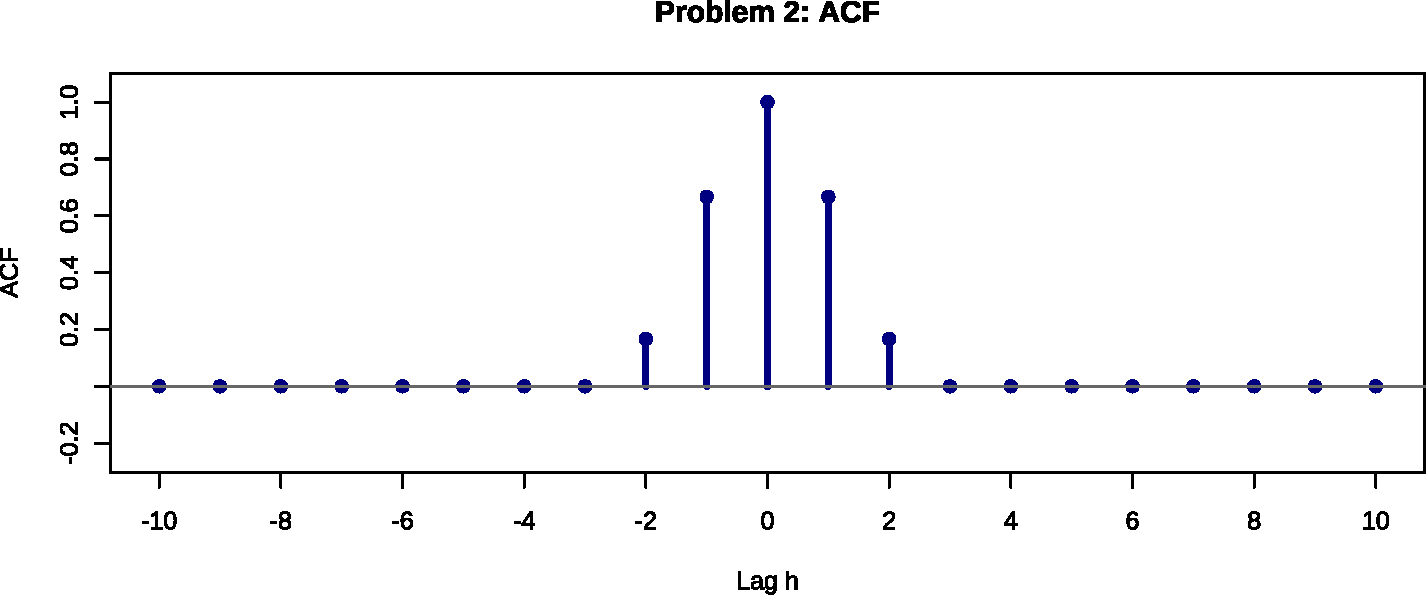
\includegraphics[width=\linewidth]{Homework5_files/figure-latex/unnamed-chunk-3-1} \end{center}

\newpage

\subsection{Problem 2 (d)}\label{problem-2-d}

\begin{problem}[Problem 2 (d)]
Is the process stationary, justify?
\end{problem}

Yes, \(\{X_t\}\) is weakly stationary because of the following:

\begin{enumerate}
\def\labelenumi{\arabic{enumi}.}
\item
  The mean function is independent of time:
  \[
  \mu_X(t) = 0 = \mu_X.
  \]
\item
  The autocovariance function depends only on lag \(h\):
  \[
  \gamma_X(t,h) = \gamma_X(h) =
  \begin{cases}
  6\sigma_w^2, & h=0,\\
  4\sigma_w^2, & h=\pm1,\\
  \sigma_w^2, & h=\pm2,\\
  0, & h \in \mathbb{Z}\setminus\{-2,-1,0,1,2\}.
  \end{cases}
  \]
\end{enumerate}

At lag \(h=0\), the ACVF is the variance, so
\[
\sigma_X^2(t) = \sigma_X^2 = \gamma_X(0) = 6\sigma_w^2,
\]
which is constant over time. Therefore, the process satisfies both conditions for weak stationarity. Hence, \(\{X_t\}\) is stationary.

\end{document}
